\par{Listing \ref{more_work_kernel} its our attempt to give every \emph{work item} more computational load, that way decreasing the
    effects of scheduling and spawning overhead of \emph{work items} and \emph{work groups}. Also this way can be studied 
    \emph{kernel's} behaviour when the cycles per \emph{work item} are increased.}

\lstinputlisting[float,caption={Kernel with more work per \emph{work item}.},label={more_work_kernel}, 
                style=customc]{/Users/clalanne/GitHubProjects/OpenCLNotes/src/code/more_work.c}

\begin{figure}[!h]
    \centering
    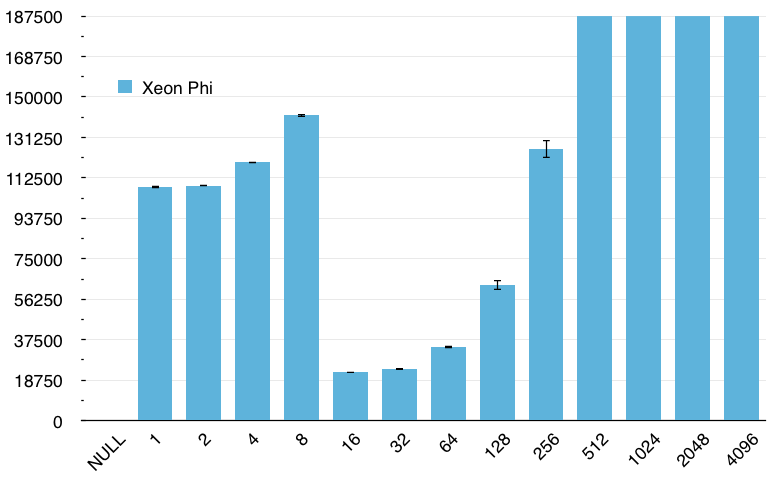
\includegraphics[width=0.49\textwidth]{figures/opt1_phi.png}
    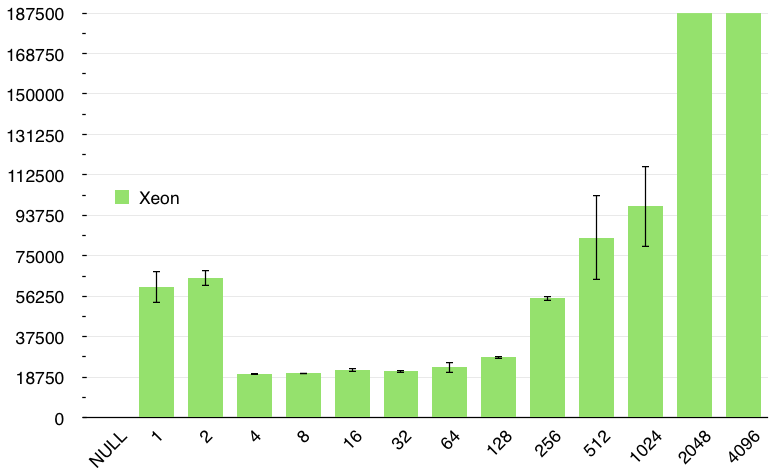
\includegraphics[width=0.49\textwidth]{figures/opt1_cpu.png}
    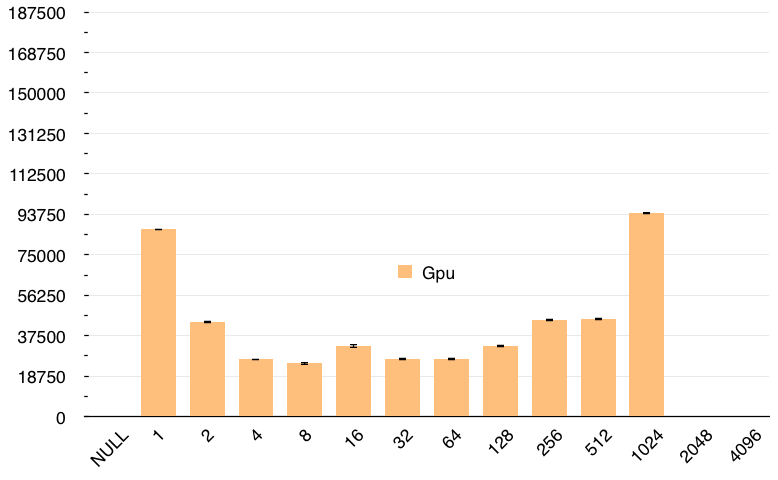
\includegraphics[width=0.49\textwidth]{figures/opt1_gpu.png}
    \caption{Matrix multiplication with more work in different architectures.}
    \label{MoreWork}
\end{figure}

\par{Figure \ref{MoreWork} shows that in the case of the Intel Xeon Phi co-processor and the Xeon CPU, the effect of vectorization
    is the same that in the previous kernel(16 for the Intel Xeon Phi and 4 for the Xeon CPU), the other interesting effect in this
    case is the performance degradation after \emph{work group} dimension 64x64 on the Intel Xeon Phi and after 128x128 on the Xeon
    CPU, clearly the Intel Xeon Phi is more sensible to the decreasing number of \emph{work groups} than the Xeon CPU, one of the 
    reasons for this is the number of \emph{computation units} available in these 2 architectures, on the Intel Xeon Phi is 236 and
    on the Xeon CPU is 40, as the number of \emph{work groups} decreased, as it is shown on table \ref{tab:work_groups}, the amount
    of available parallelism that take advantage of the \emph{comput units} available in these 2 architectures decreases as well.}


\begin{table}[!h]
    \centering
    \begin{tabular}{| l | l | l | l |}
    \hline
    \emph{Work Group} Dimension & \#\emph{Work Groups} \\ \hline
    16x16 & 65536 \\ \hline
    32x32 & 16384 \\ \hline
    64x64 & 4096 \\ \hline
    128x128 & 1024 \\ \hline
    256x256 & 256 \\ \hline
    512x512 & 64 \\ \hline
    1024x1024 & 16 \\ \hline
    2048x2048 & 4 \\ \hline
    4096x4096 & 1 \\ 
    \hline
    \end{tabular}
    \caption{\emph{Work group} dimension versus numbers of \emph{work groups}.}
    \label{tab:work_groups}
\end{table}

\par{In this case the most performant of the 3 architectures analized is the Xeon as its shown on figure\ref{MoreWorkComp} and 
    we cannot see any advantage in comparison with the naive \emph{kernel} using more load per \emph{work item}.}


